\documentclass[aspectratio=169, 11pt]{beamer}

\usetheme{Madrid}
\usecolortheme{default}

\usepackage[utf8]{inputenc}
\usepackage[T1]{fontenc}
\usepackage{lmodern}
\usepackage{amsmath,amssymb}
\usepackage{booktabs}
\usepackage{graphicx}
\usepackage{tikz}
\usepackage{pgfplots}
\usepackage{hyperref}
\usepackage{xcolor}

\pgfplotsset{compat=1.18}

\definecolor{shanghaitech}{RGB}{100, 30, 60}
\setbeamercolor{palette primary}{bg=shanghaitech, fg=white}
\setbeamercolor{palette secondary}{bg=shanghaitech!80, fg=white}
\setbeamercolor{palette tertiary}{bg=shanghaitech!60, fg=white}
\setbeamercolor{structure}{fg=shanghaitech}
\setbeamercolor{title}{fg=white, bg=shanghaitech}
\setbeamercolor{frametitle}{fg=white, bg=shanghaitech}

\title[Rail Line Planning]{Reproducing Classical Heuristics for\\Urban Rail Transit Line Planning}
\subtitle{Laporte 2005 \& Ahmed 2020}
\author[Yang et al.]{Zaizhou Yang, Yuzhou Lu, Jingrong Guan}
\institute[ShanghaiTech]{ShanghaiTech University\\CS240 -- Algorithm Design and Analysis}
\date{June 2026}

\setbeamertemplate{footline}{
  \leavevmode%
  \hbox{%
    \begin{beamercolorbox}[wd=.333333\paperwidth,ht=2.5ex,dp=1ex,center]{author in head/foot}%
      \usebeamerfont{author in head/foot}\insertshortauthor
    \end{beamercolorbox}%
    \begin{beamercolorbox}[wd=.333333\paperwidth,ht=2.5ex,dp=1ex,center]{title in head/foot}%
      \usebeamerfont{title in head/foot}\insertshorttitle
    \end{beamercolorbox}%
    \begin{beamercolorbox}[wd=.333333\paperwidth,ht=2.5ex,dp=1ex,right]{date in head/foot}%
      \usebeamerfont{date in head/foot}\insertshortdate{}\hspace*{2em}
      \insertframenumber{} / \inserttotalframenumber\hspace*{2ex}
    \end{beamercolorbox}}%
  \vskip0pt%
}

\graphicspath{{./}{../../line_network_model/output/}}

\begin{document}

%-----------------------------------------------------------------------
\begin{frame}
\titlepage
\end{frame}

%-----------------------------------------------------------------------
\begin{frame}{Outline}
\tableofcontents
\end{frame}

%=======================================================================
\section{Introduction}
%=======================================================================

%-----------------------------------------------------------------------
\begin{frame}{The Transit Network Design Problem (TNDP)}

\begin{itemize}
    \item Design an urban rail transit network: \textbf{where to build stations} and \textbf{how to connect them}.
    \item Combines station location, alignment planning, and network topology under constraints:
    \begin{itemize}
        \item Construction budgets
        \item Population/trip coverage
        \item Geometric feasibility (non-intersection, spacing)
    \end{itemize}
    \item NP-hard in the general case \(\Rightarrow\) practical heuristics needed.
\end{itemize}

\vspace{0.3cm}
\begin{block}{Our Goal}
Reproduce two representative algorithms and evaluate them on a Shanghai dataset with 54 candidate stations.
\end{block}
\end{frame}

%-----------------------------------------------------------------------
\begin{frame}{Overview of the Two Papers}

\begin{columns}[T]
\begin{column}{0.48\textwidth}
\begin{block}{Paper 1: Laporte et al.\ 2005}
\small
\textit{``Maximizing Trip Coverage in the Location of a Single Rapid Transit Alignment''}
\begin{itemize}
    \item Single line
    \item Maximize OD coverage
    \item Greedy heuristics
    \item Polynomial-time
\end{itemize}
\end{block}
\end{column}
\begin{column}{0.48\textwidth}
\begin{block}{Paper 2: Ahmed et al.\ 2020}
\small
\textit{``GIS and Genetic Algorithm Based Integrated Optimization for Rail Transit System Planning''}
\begin{itemize}
    \item Multi-line network
    \item Minimize total system cost
    \item Genetic algorithm
    \item GIS integration
\end{itemize}
\end{block}
\end{column}
\end{columns}
\end{frame}

%-----------------------------------------------------------------------
\begin{frame}{Candidate Station Selection (Shanghai)}

\begin{columns}[T]
\begin{column}{0.55\textwidth}
\begin{itemize}
    \item 54 candidate stations in central Shanghai
    \item Selected from 4 spatial data layers:
    \begin{itemize}
        \item Population centers
        \item Job centers
        \item Transport hubs
        \item Commercial centers
    \end{itemize}
    \item Data source: OpenStreetMap
    \item Corridor graph built for alignment search
\end{itemize}
\end{column}
\begin{column}{0.42\textwidth}

\includegraphics[width=\textwidth]{01_station_selection.png}
\end{column}
\end{columns}
\end{frame}

%=======================================================================
\section{Paper 1: Laporte 2005}
%=======================================================================

%-----------------------------------------------------------------------
\begin{frame}{Laporte 2005 -- Problem Formulation}

\textbf{MTCP} (Maximal Trip Coverage Problem):

\begin{itemize}
    \item Build \textbf{one non-intersecting path} through candidate stations
    \item Maximize total OD trip coverage
    \item Subject to a \textbf{length budget} \(L_{\max}\)
\end{itemize}

\vspace{0.3cm}
\[
\max \sum_{(i,j) \in OD} f_{ij} \cdot \mathbf{1}[\text{trip } (i,j) \text{ is covered}]
\]
\[
\text{s.t.} \quad \text{total line length} \leq L_{\max}
\]

\begin{itemize}
    \item Generalizes bounded-length Hamiltonian path \(\Rightarrow\) \textbf{NP-hard}
    \item \(f_{ij}\): gravity-model OD demand between stations \(i\) and \(j\)
\end{itemize}
\end{frame}

%-----------------------------------------------------------------------
\begin{frame}{Laporte 2005 -- Heuristics}

\begin{columns}[T]
\begin{column}{0.48\textwidth}
\begin{block}{H1: Greedy Extension}
\begin{enumerate}
    \item Start from a seed edge
    \item Extend at either endpoint
    \item Pick the node with highest marginal coverage gain
    \item Repeat until budget exhausted
\end{enumerate}
\vspace{0.15cm}
\small
\textbf{Complexity:} \(O(n^2 \cdot |E|^2)\)
\end{block}
\end{column}
\begin{column}{0.48\textwidth}
\begin{block}{H2: Greedy Insertion}
\begin{enumerate}
    \item Start from a seed edge
    \item Insert new node at \emph{any} position in path
    \item Pick (node, position) with highest gain
    \item Repeat until budget exhausted
\end{enumerate}
\vspace{0.15cm}
\small
\textbf{Complexity:} \(O(n^2 \cdot |E|^3)\)

\smallskip
Three variants: \textbf{H2-A} (max ridership), \textbf{H2-B} (min length), \textbf{H2-C} (max ratio)
\end{block}
\end{column}
\end{columns}

\vspace{0.2cm}
\textbf{Post-optimization}: local search swaps to improve an existing solution.
\end{frame}

%-----------------------------------------------------------------------
\begin{frame}{Laporte 2005 -- Results on Shanghai Data}

\centering
\small
\begin{tabular}{lcccc}
\toprule
\textbf{Heuristic} & \textbf{Length (km)} & \textbf{Stations} & \textbf{Ridership} & \textbf{Time (s)} \\
\midrule
\multicolumn{5}{c}{\(L_{\max} = 60\) km} \\
\midrule
H1 (Extension)     & 59.8 & 18 & 6.22e12 & 0.05 \\
H2-A (Insertion)   & 59.9 & 31 & 1.37e13 & 0.79 \\
H2-A + post-opt    & 59.9 & 31 & 1.37e13 & 0.02 \\
H2-B (Insertion)   & 59.9 & 36 & 9.57e12 & 1.04 \\
H2-C (Insertion)   & 59.6 & 33 & 1.36e13 & 0.93 \\
\bottomrule
\end{tabular}

\vspace{0.3cm}
\begin{itemize}
    \item H2 variants select \textbf{more stations} (31--36 vs.\ 18) within the same budget.
    \item H2-A achieves \(\sim\)2.2\(\times\) the ridership of H1.
    \item Post-optimization provides marginal improvement on this dataset.
\end{itemize}
\end{frame}

%-----------------------------------------------------------------------
\begin{frame}{Laporte 2005 -- Alignment Visualizations}

\begin{columns}[T]
\begin{column}{0.48\textwidth}
\centering
\small H1: Greedy Extension\\[0.2cm]
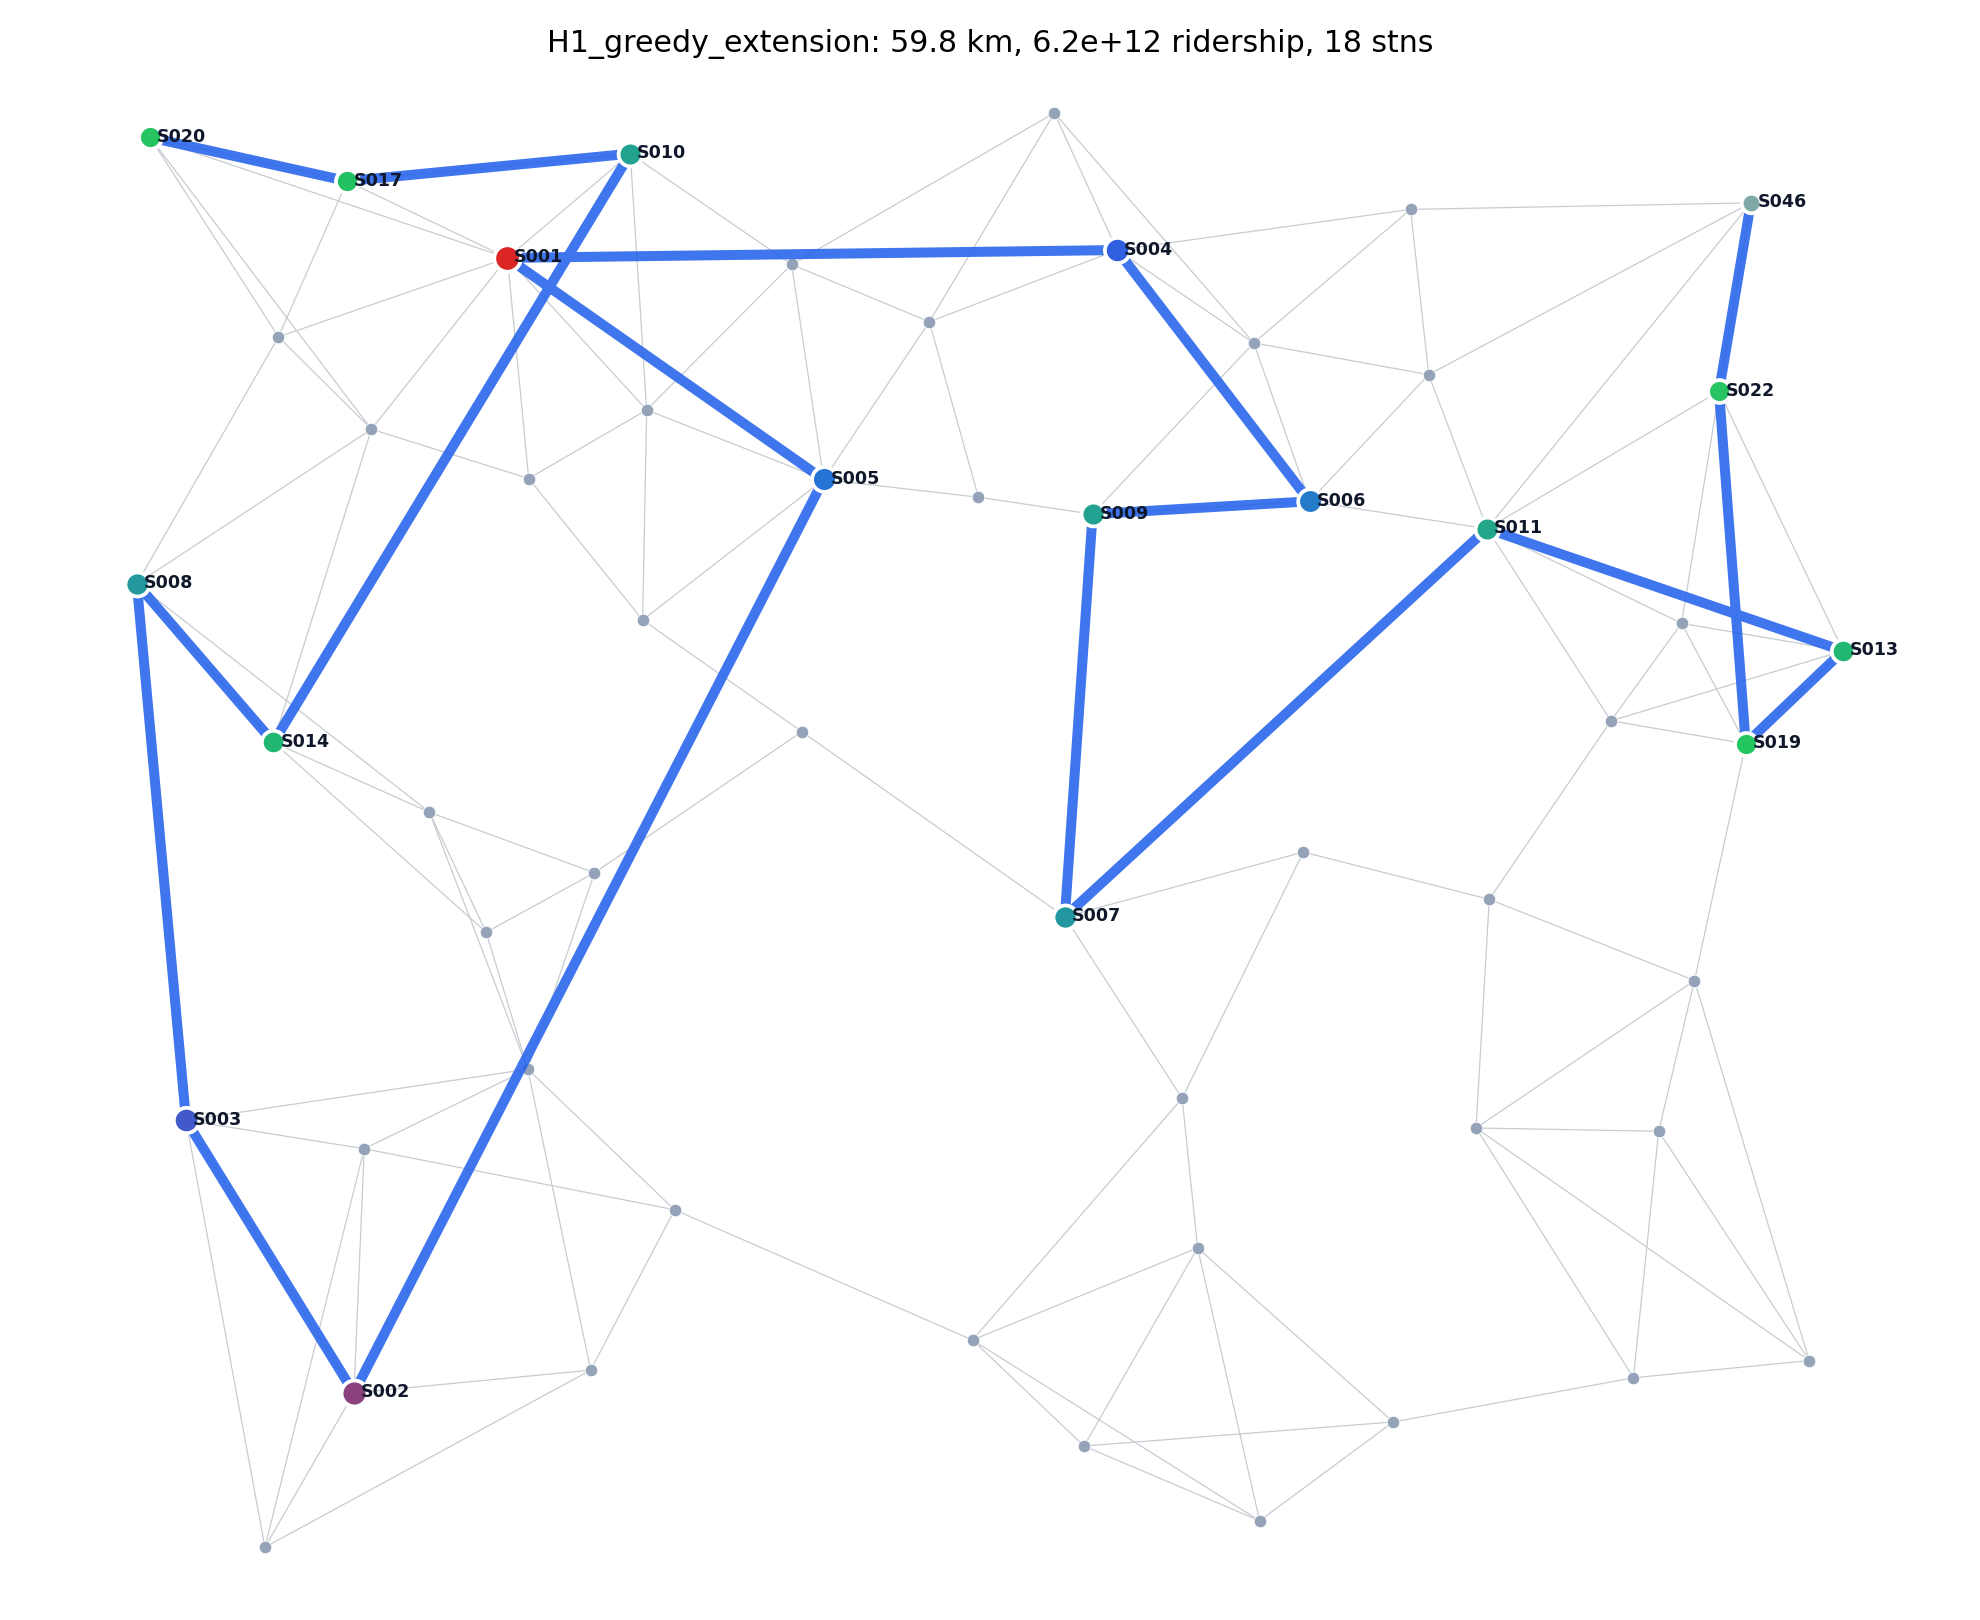
\includegraphics[width=\textwidth]{laporte2005_reproduction/alignment_lmax60_h1}
\end{column}
\begin{column}{0.48\textwidth}
\centering
\small H2-A: Greedy Insertion\\[0.2cm]
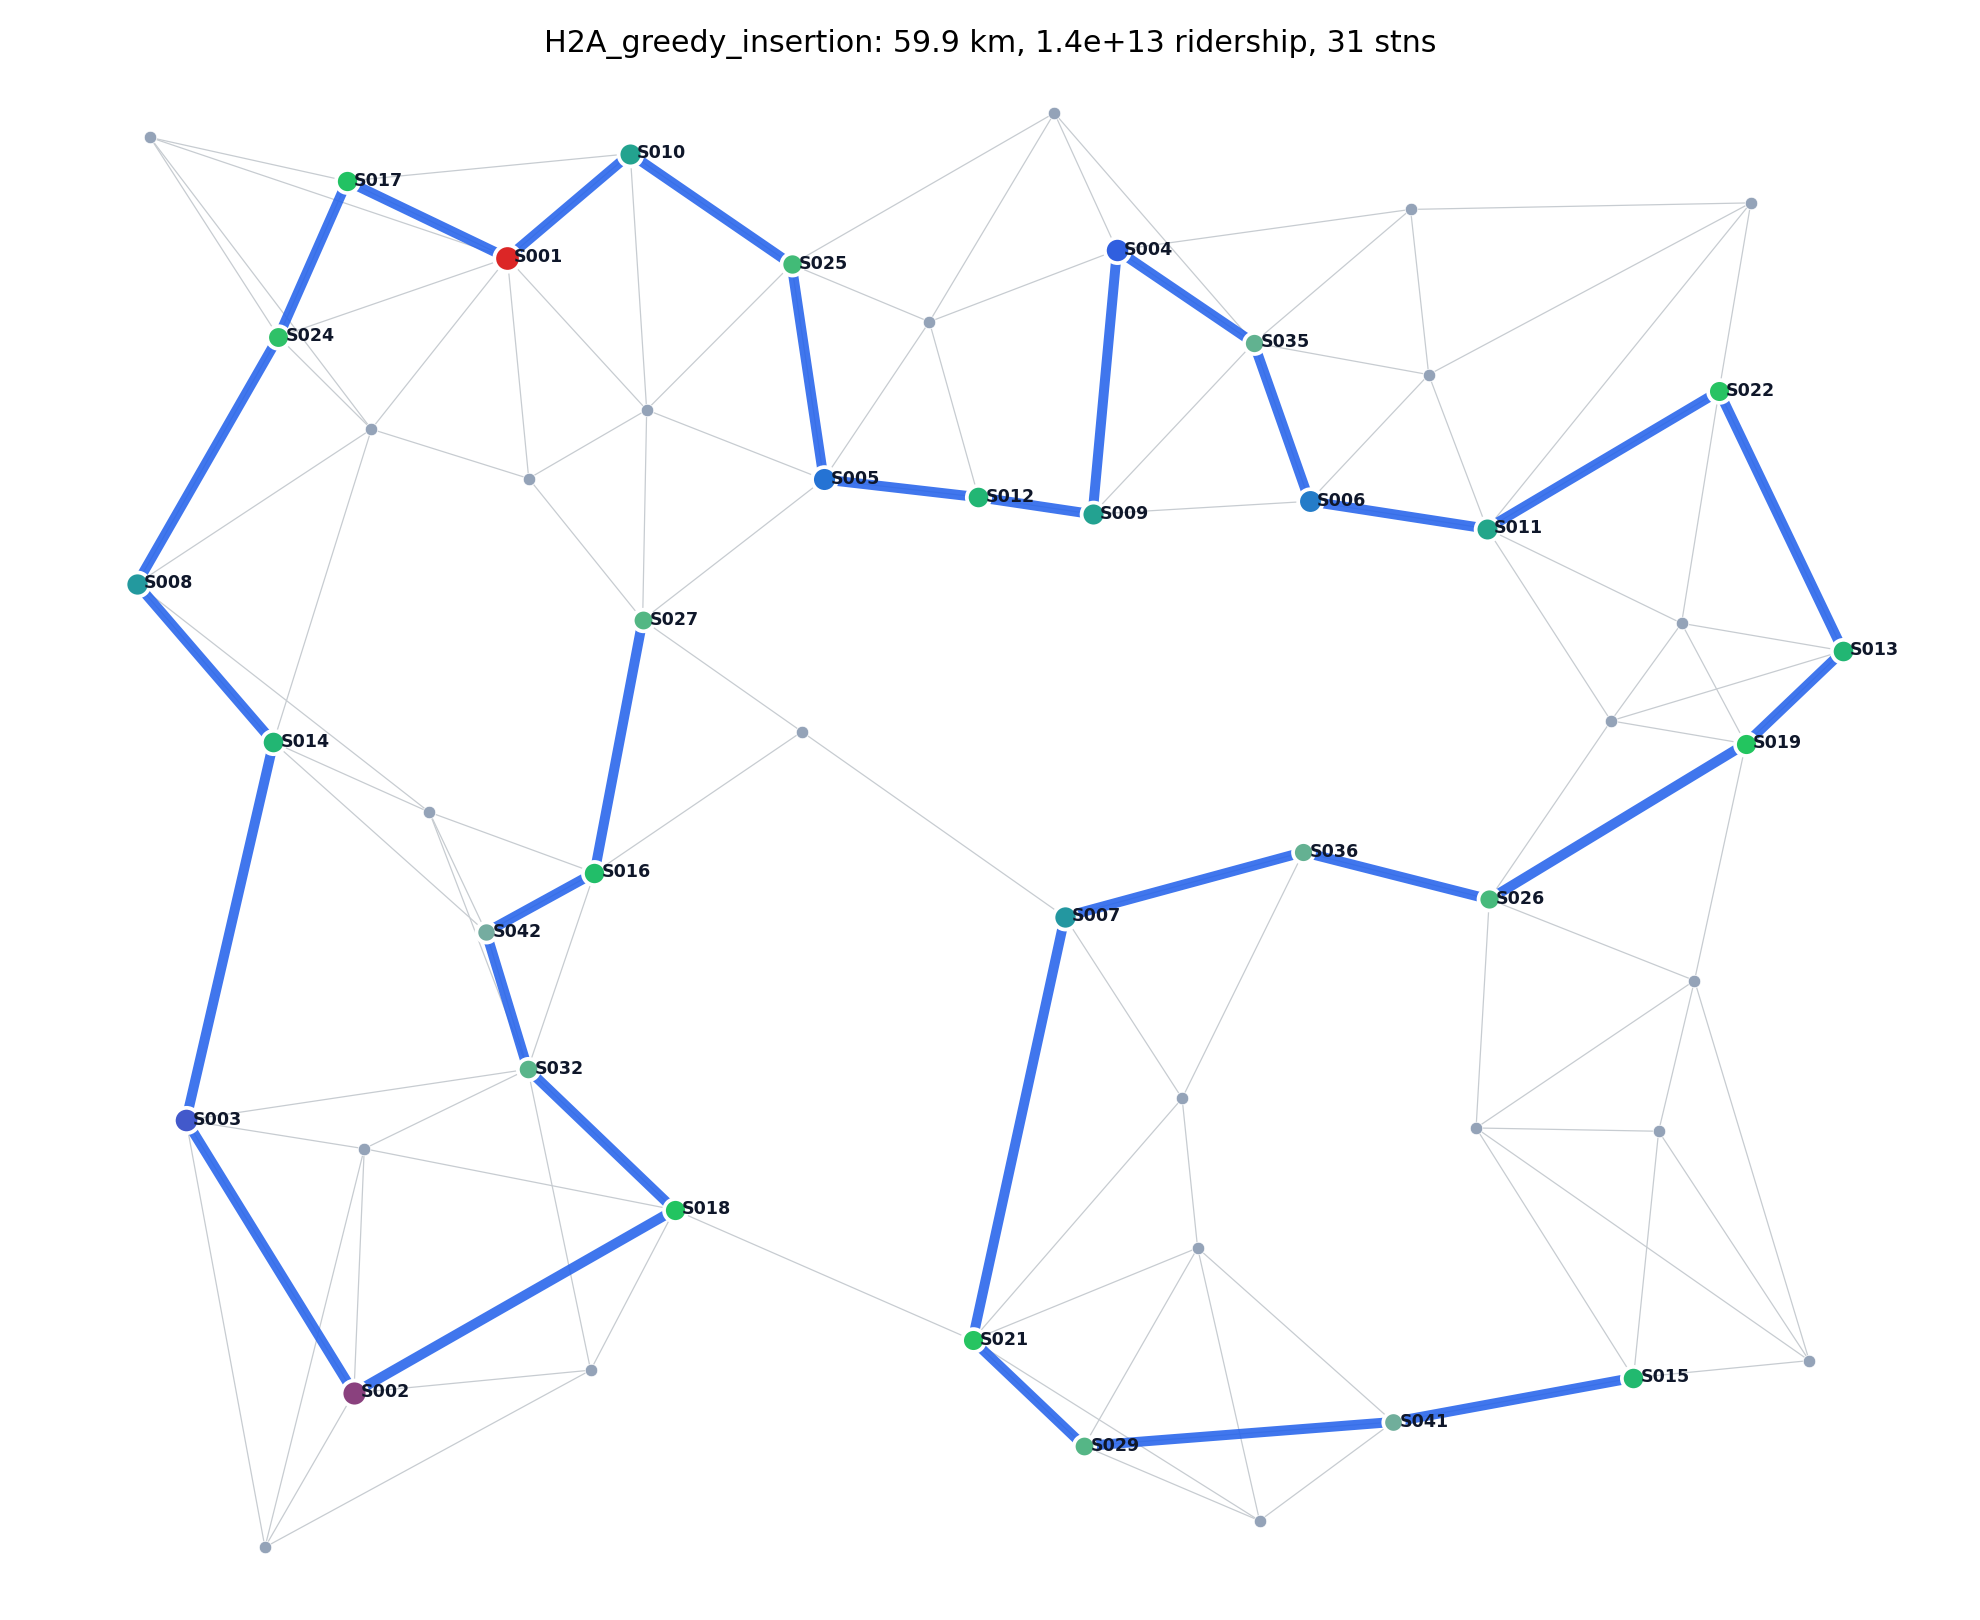
\includegraphics[width=\textwidth]{laporte2005_reproduction/alignment_lmax60_h2a}
\end{column}
\end{columns}
\end{frame}

%-----------------------------------------------------------------------
\begin{frame}{Laporte 2005 -- Spacing Sensitivity}

\begin{columns}[T]
\begin{column}{0.55\textwidth}
\begin{itemize}
    \item Varying min inter-station spacing: 500m -- 1500m
    \item Paper claims: H1 dominates for spacing \(\geq\) 1250m
    \item On Shanghai data: \textbf{H2-A consistently outperforms H1} across all spacing values
    \item Denser candidate set (54 stations, avg.\ \(\sim\)1km) means H2's insertion flexibility helps even at tight spacing
\end{itemize}
\end{column}
\begin{column}{0.42\textwidth}
\centering
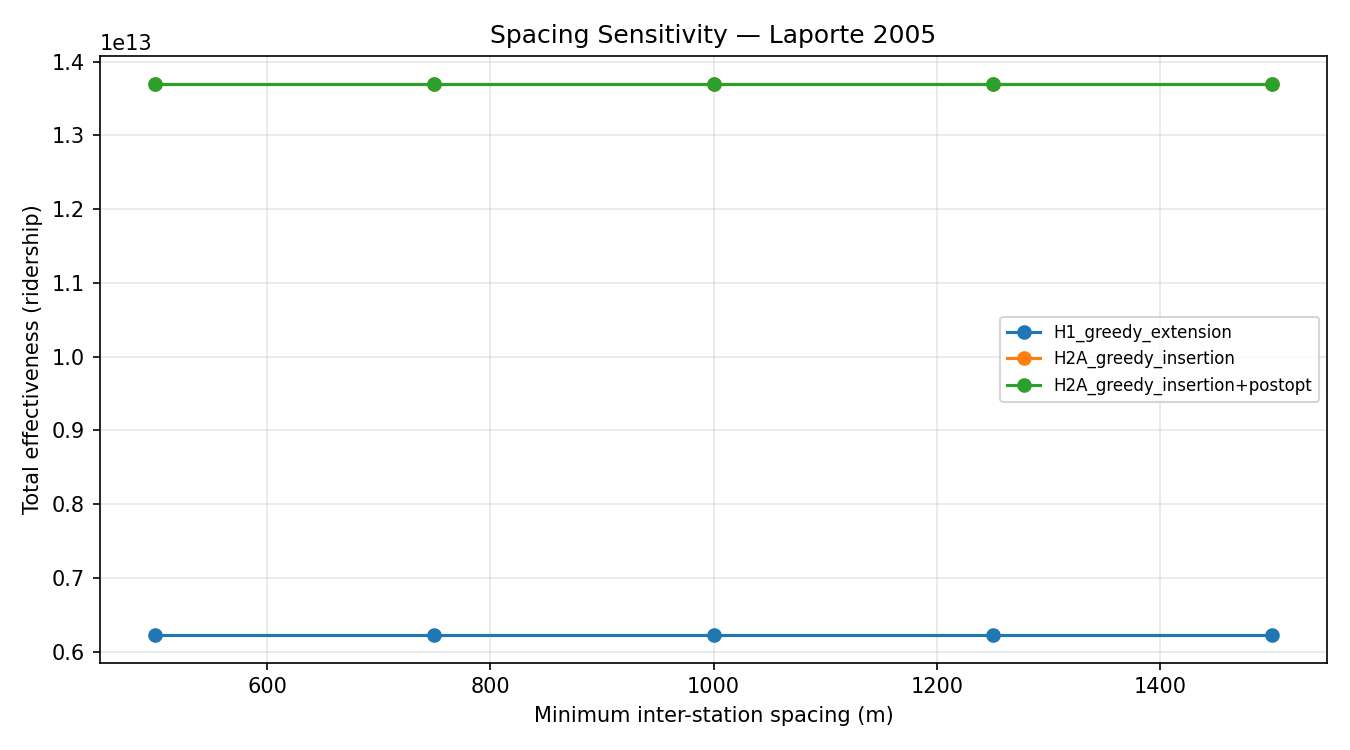
\includegraphics[width=\textwidth]{laporte2005_reproduction/spacing_sensitivity}
\end{column}
\end{columns}
\end{frame}

%-----------------------------------------------------------------------
\begin{frame}{Laporte 2005 -- Runtime Scalability}

\begin{columns}[T]
\begin{column}{0.55\textwidth}
\begin{itemize}
    \item Sweep \(n \in \{20, 30, 40, 50, 60, 80, 100\}\) stations
    \item H1: \(\sim\)0.8s at \(n=100\)
    \item H2-A/H2-C: \(\sim\)20s at \(n=100\)
    \item Confirms polynomial scaling
    \item H1 is \(\sim\)25\(\times\) faster than H2 at \(n=100\)
\end{itemize}
\end{column}
\begin{column}{0.42\textwidth}
\centering
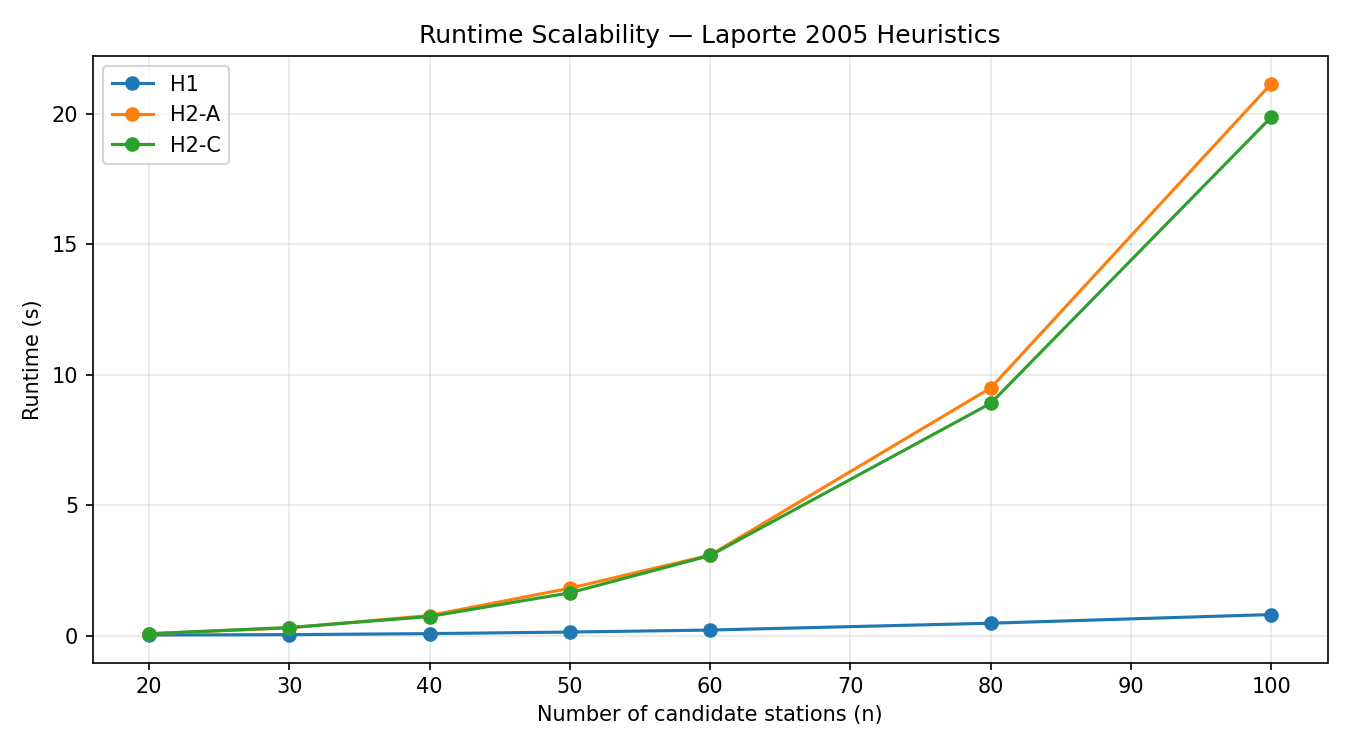
\includegraphics[width=\textwidth]{laporte2005_reproduction/runtime_scalability}
\end{column}
\end{columns}
\end{frame}

%=======================================================================
\section{Paper 2: Ahmed 2020}
%=======================================================================

%-----------------------------------------------------------------------
\begin{frame}{Ahmed 2020 -- Problem Formulation}

\textbf{Multi-line rail transit network design}:

\begin{itemize}
    \item Simultaneously select stations \textbf{and} line network
    \item Minimize total system cost:
\end{itemize}

\[
\min \quad \phi_p \cdot C_{\text{passenger}} + \phi_o \cdot C_{\text{operator}} + \phi_c \cdot C_{\text{community}}
\]

\begin{itemize}
    \item \(C_{\text{passenger}}\): travel time savings vs.\ car/bus
    \item \(C_{\text{operator}}\): operating cost savings from mode shift
    \item \(C_{\text{community}}\): construction cost (alignment + stations)
\end{itemize}

\begin{block}{Key Insight}
Simultaneous optimization of all lines \(\approx\) \textbf{70\% better} than optimizing lines individually.
\end{block}
\end{frame}

%-----------------------------------------------------------------------
\begin{frame}{Ahmed 2020 -- Two-Stage Approach}

\begin{columns}[T]
\begin{column}{0.45\textwidth}
\begin{block}{Stage 1: Feasibility Screening}
\begin{itemize}
    \item GIS-based spatial filtering
    \item Our adaptation: reuse the 54-station pipeline (population, jobs, transport, commercial layers)
    \item Produces candidate station pool
\end{itemize}
\end{block}
\end{column}
\begin{column}{0.50\textwidth}
\begin{block}{Stage 2: Genetic Algorithm}
\begin{itemize}
    \item \textbf{Chromosome}: sequence of station indices per line
    \item \textbf{Fixed terminals}: selected from high-OD station pairs
    \item \textbf{Operators}:
    \begin{itemize}
        \item Tournament selection (size 2)
        \item Uniform crossover (\(P_c = 0.7\))
        \item Station-level mutation (\(P_m = 0.3\))
    \end{itemize}
    \item \textbf{Feasibility repair} after crossover/mutation
\end{itemize}
\end{block}
\end{column}
\end{columns}
\end{frame}

%-----------------------------------------------------------------------
\begin{frame}{Ahmed 2020 -- GA Design Details}

\begin{columns}[T]
\begin{column}{0.48\textwidth}
\begin{block}{Chromosome Encoding}
\small
\texttt{[Line\_1\_genes, Line\_2\_genes, \ldots]}

\texttt{Line\_k = [term\_a, stations..., term\_b]}

Each gene = station index from candidate pool.
\end{block}

\begin{block}{Constraints}
\small
\begin{itemize}
    \item 4--10 stations per line
    \item Min spacing: 1000m
    \item Max spacing: 3000m
    \item Max overlap: 30\%
\end{itemize}
\end{block}
\end{column}
\begin{column}{0.48\textwidth}
\begin{block}{GA Parameters}
\small
\begin{tabular}{ll}
\toprule
\textbf{Parameter} & \textbf{Value} \\
\midrule
Population size & 500 \\
Generations & 50 \\
Crossover rate \(P_c\) & 0.7 \\
Mutation rate \(P_m\) & 0.3 \\
Tournament size & 2 \\
\bottomrule
\end{tabular}
\end{block}

\begin{block}{Fitness}
\small
\(\min \phi_p C_p + \phi_o C_o + \phi_c C_c\)

Negative cost = savings (good).
\end{block}
\end{column}
\end{columns}
\end{frame}

%-----------------------------------------------------------------------
\begin{frame}{Ahmed 2020 -- GA Convergence}

\begin{columns}[T]
\begin{column}{0.32\textwidth}
\centering
\small 1-line\\[0.2cm]
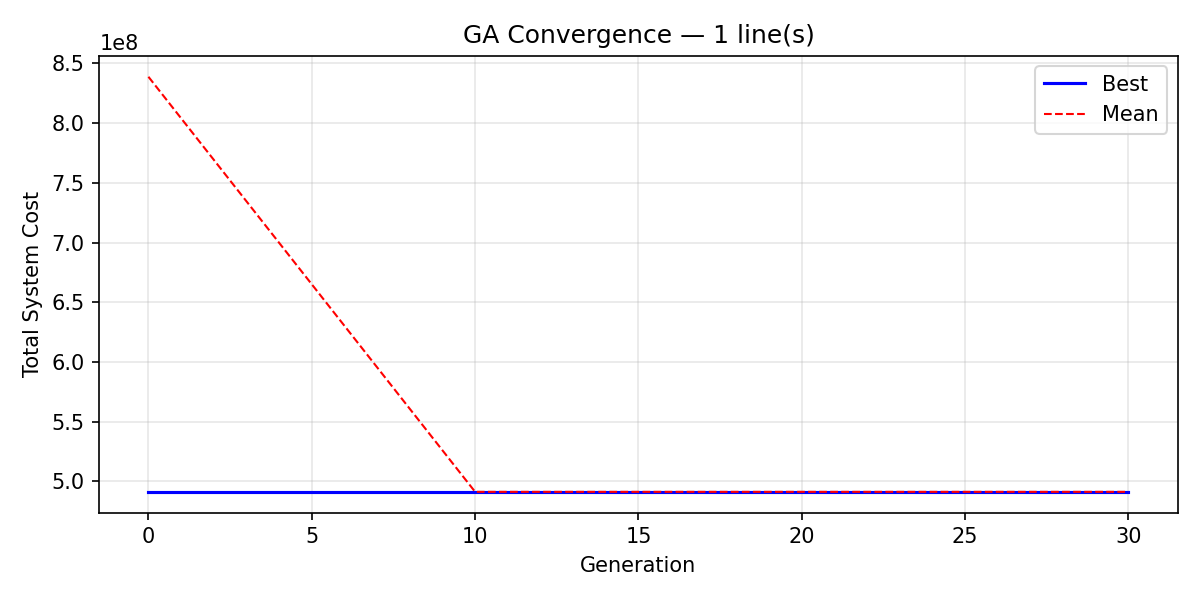
\includegraphics[width=\textwidth]{ahmed2020_reproduction/convergence_1line}
\end{column}
\begin{column}{0.32\textwidth}
\centering
\small 2-line\\[0.2cm]
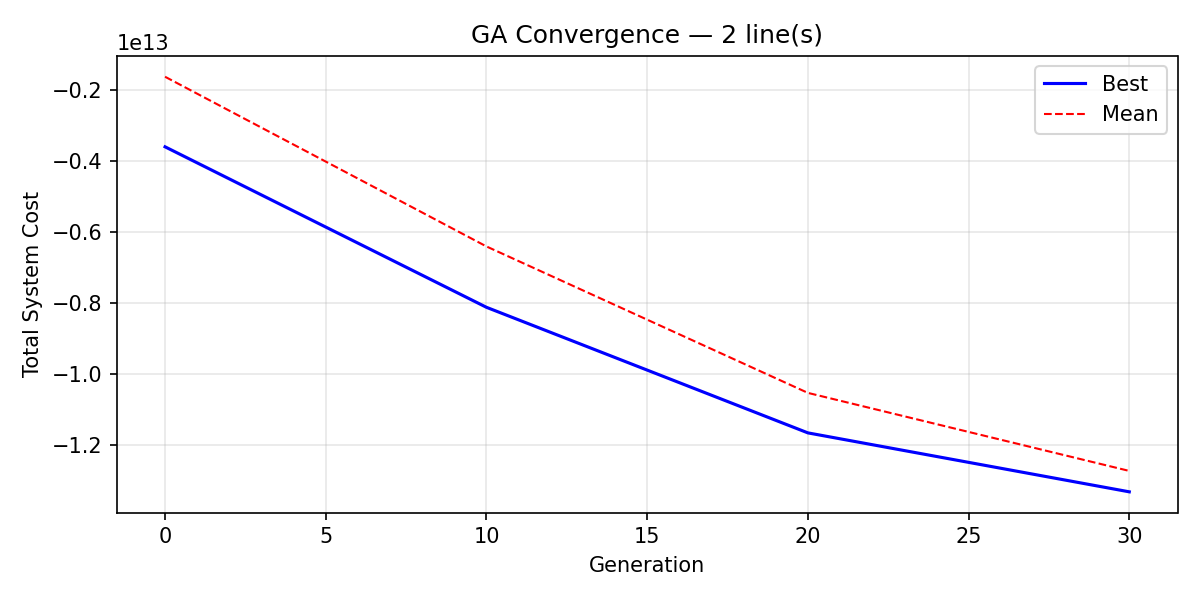
\includegraphics[width=\textwidth]{ahmed2020_reproduction/convergence_2line}
\end{column}
\begin{column}{0.32\textwidth}
\centering
\small 3-line\\[0.2cm]
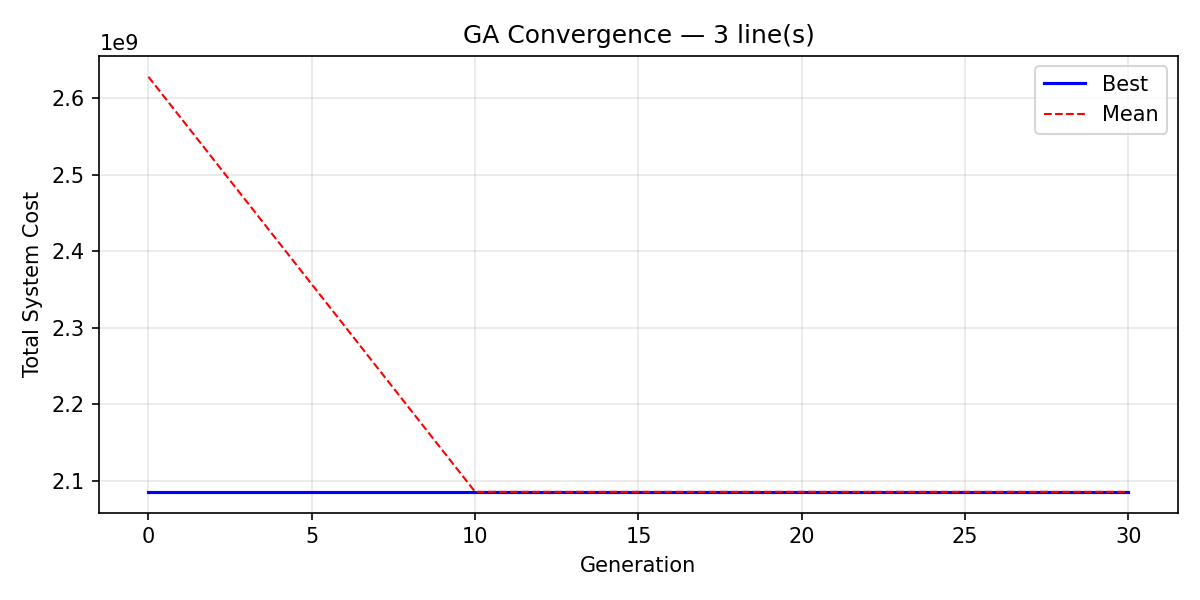
\includegraphics[width=\textwidth]{ahmed2020_reproduction/convergence_3line}
\end{column}
\end{columns}

\vspace{0.3cm}
\begin{itemize}
    \item Convergence within 20--30 generations for all scenarios.
    \item 2-line achieves lowest total cost (\(-1.33\times10^{13}\)).
\end{itemize}
\end{frame}

%-----------------------------------------------------------------------
\begin{frame}{Ahmed 2020 -- Network Visualizations}

\begin{columns}[T]
\begin{column}{0.48\textwidth}
\centering
\small 1-line network (14 stations, 37.0 km)\\[0.2cm]
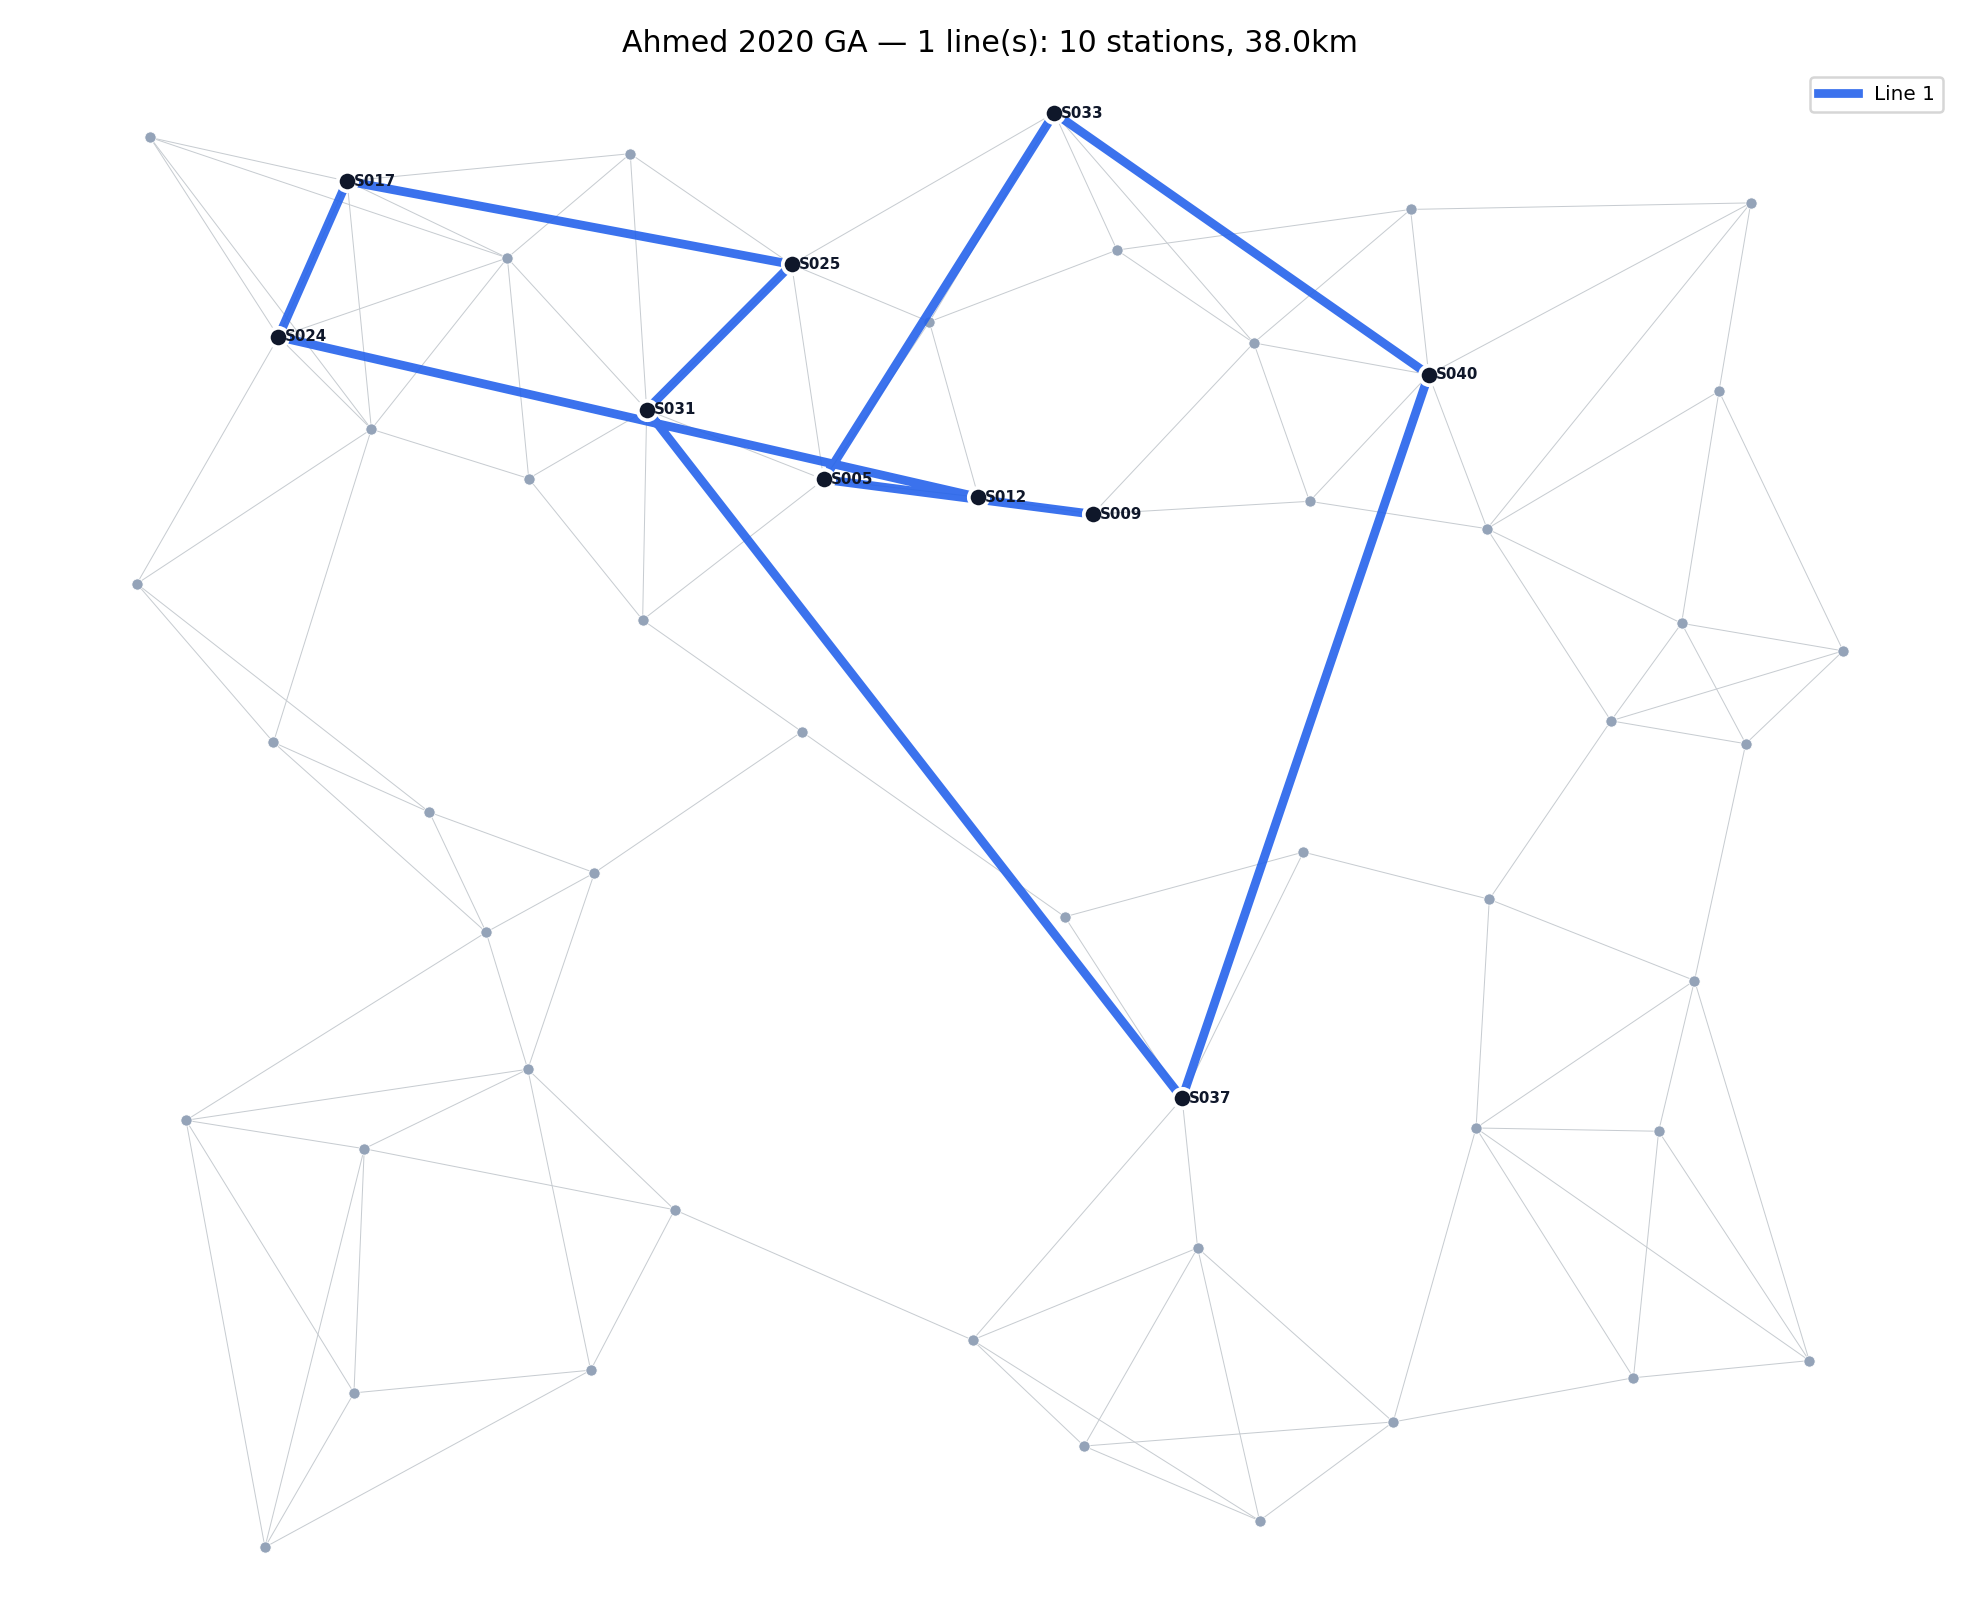
\includegraphics[width=\textwidth]{ahmed2020_reproduction/network_1line}
\end{column}
\begin{column}{0.48\textwidth}
\centering
\small 2-line network (23 stations, 85.7 km)\\[0.2cm]
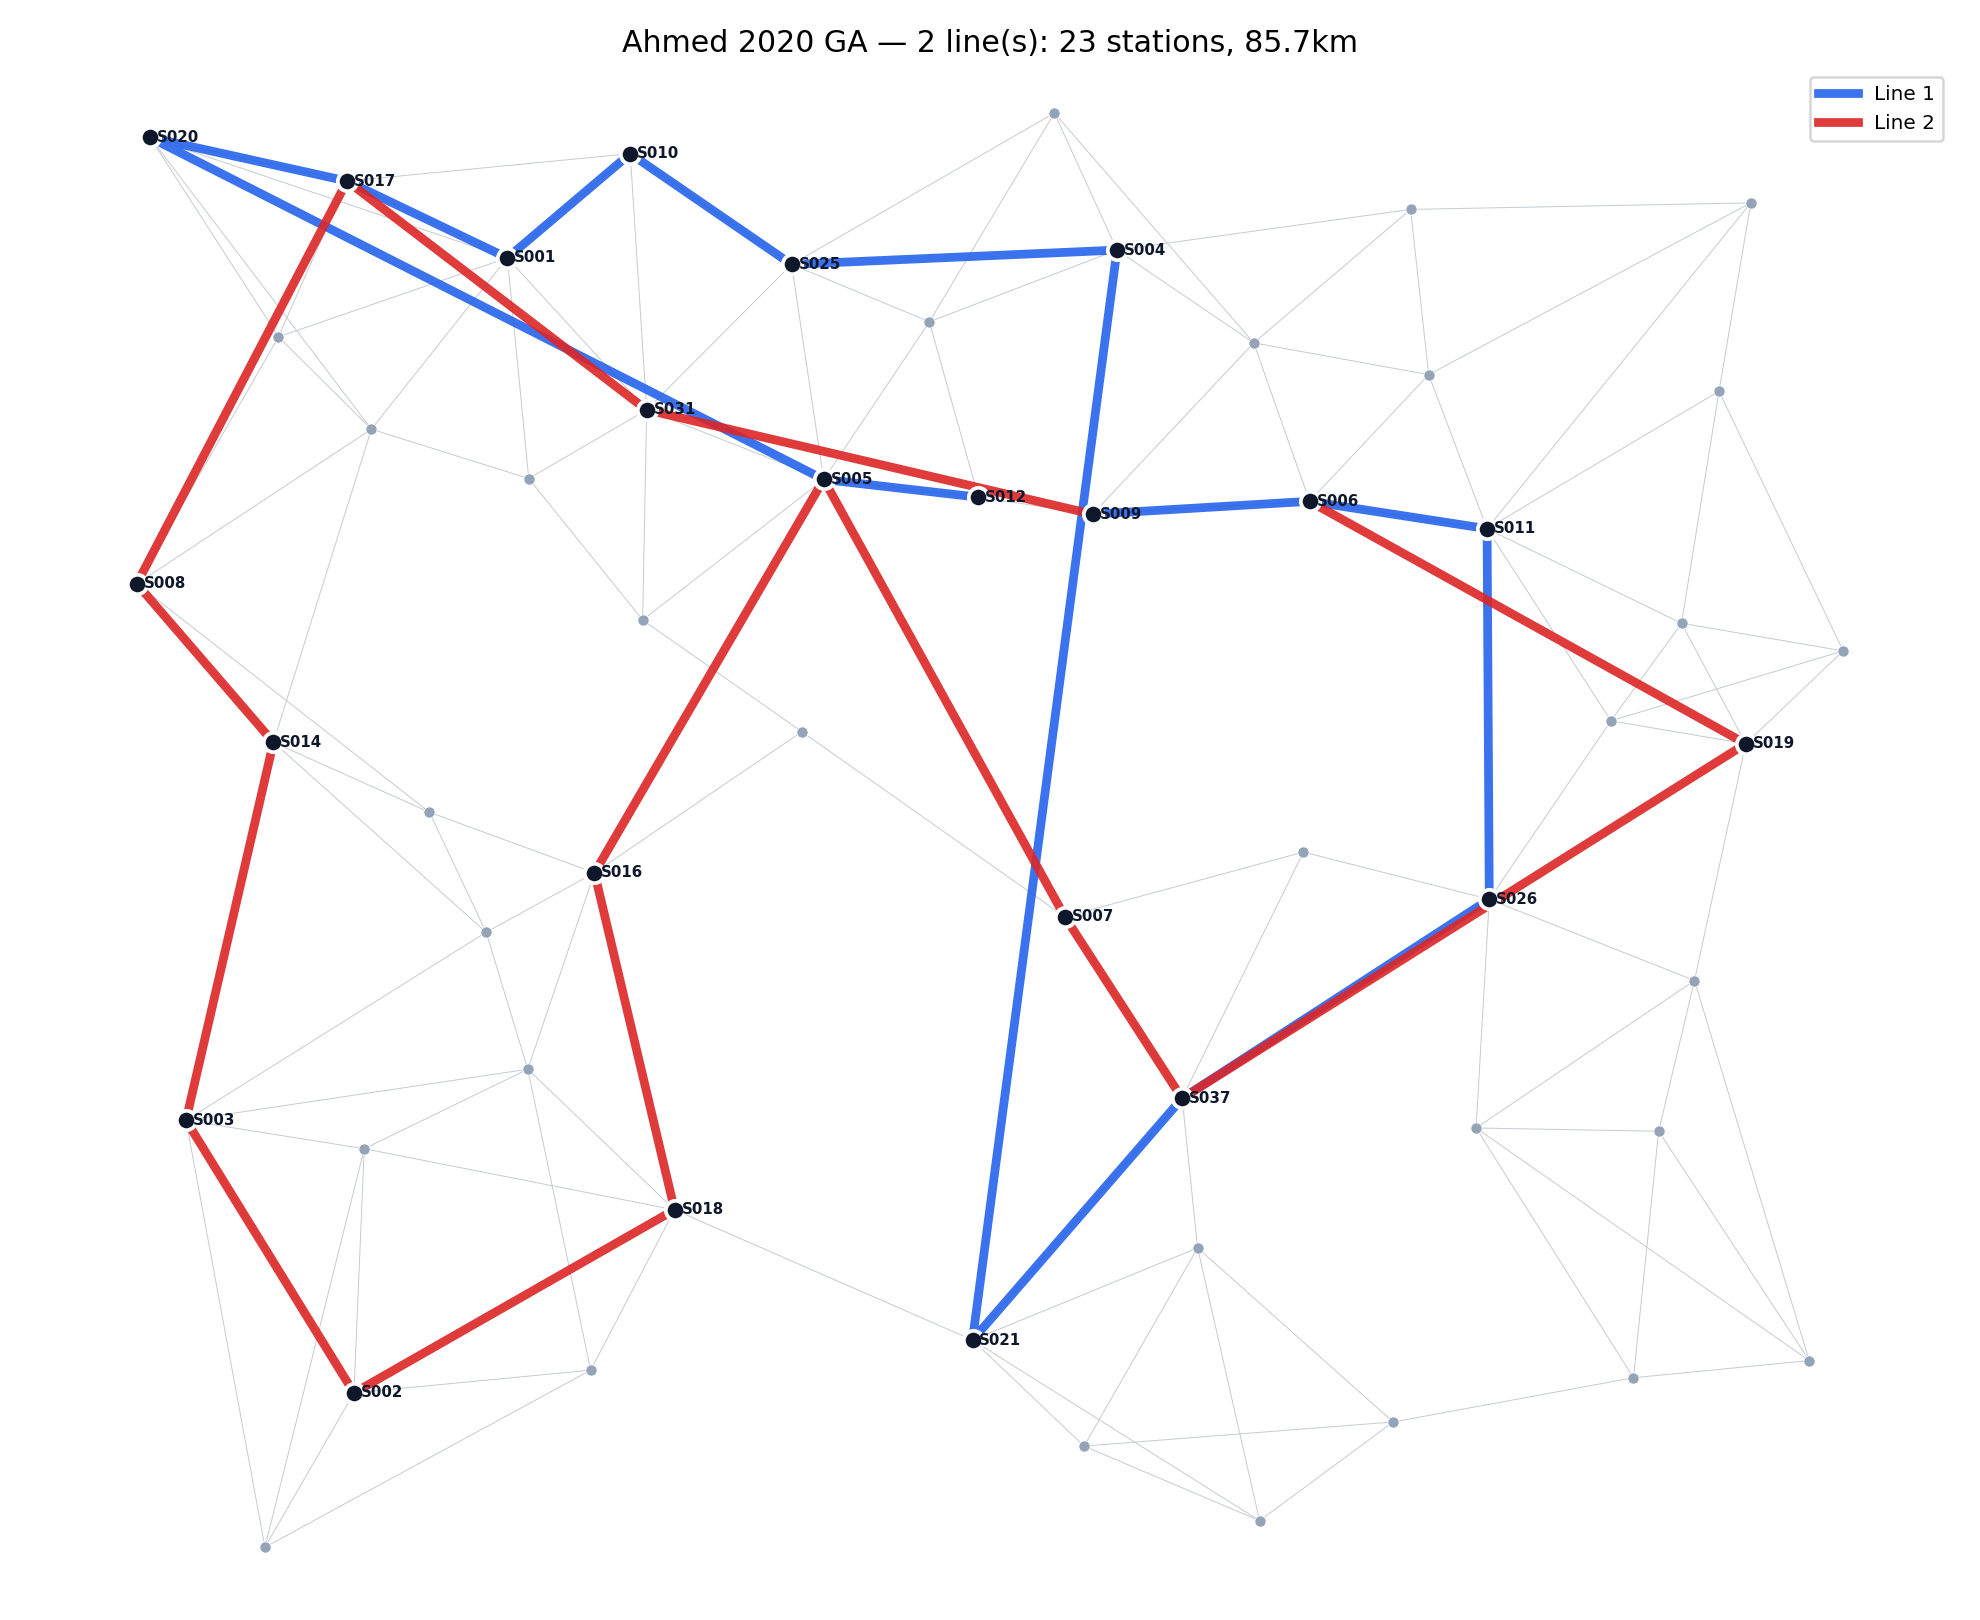
\includegraphics[width=\textwidth]{ahmed2020_reproduction/network_2line}
\end{column}
\end{columns}
\end{frame}

%-----------------------------------------------------------------------
\begin{frame}{Ahmed 2020 -- Simultaneous vs.\ Individual}

\begin{columns}[T]
\begin{column}{0.55\textwidth}
\centering
\small
\begin{tabular}{lcc}
\toprule
& \textbf{Simultaneous} & \textbf{Individual} \\
\midrule
Total cost & \(-1.33\times10^{13}\) & \(-1.13\times10^{13}\) \\
Stations & 23 & 28 \\
Length (km) & 85.7 & 80.1 \\
Runtime (s) & 58.3 & 68.9 \\
\bottomrule
\end{tabular}

\vspace{0.3cm}
\textbf{18\% improvement} from simultaneous optimization.

\smallskip
\small
(Paper reports 70\% -- difference due to simplified cost model and smaller candidate set.)
\end{column}
\begin{column}{0.42\textwidth}
\centering
\small 3-line network (20 stations, 130.8 km)\\[0.2cm]
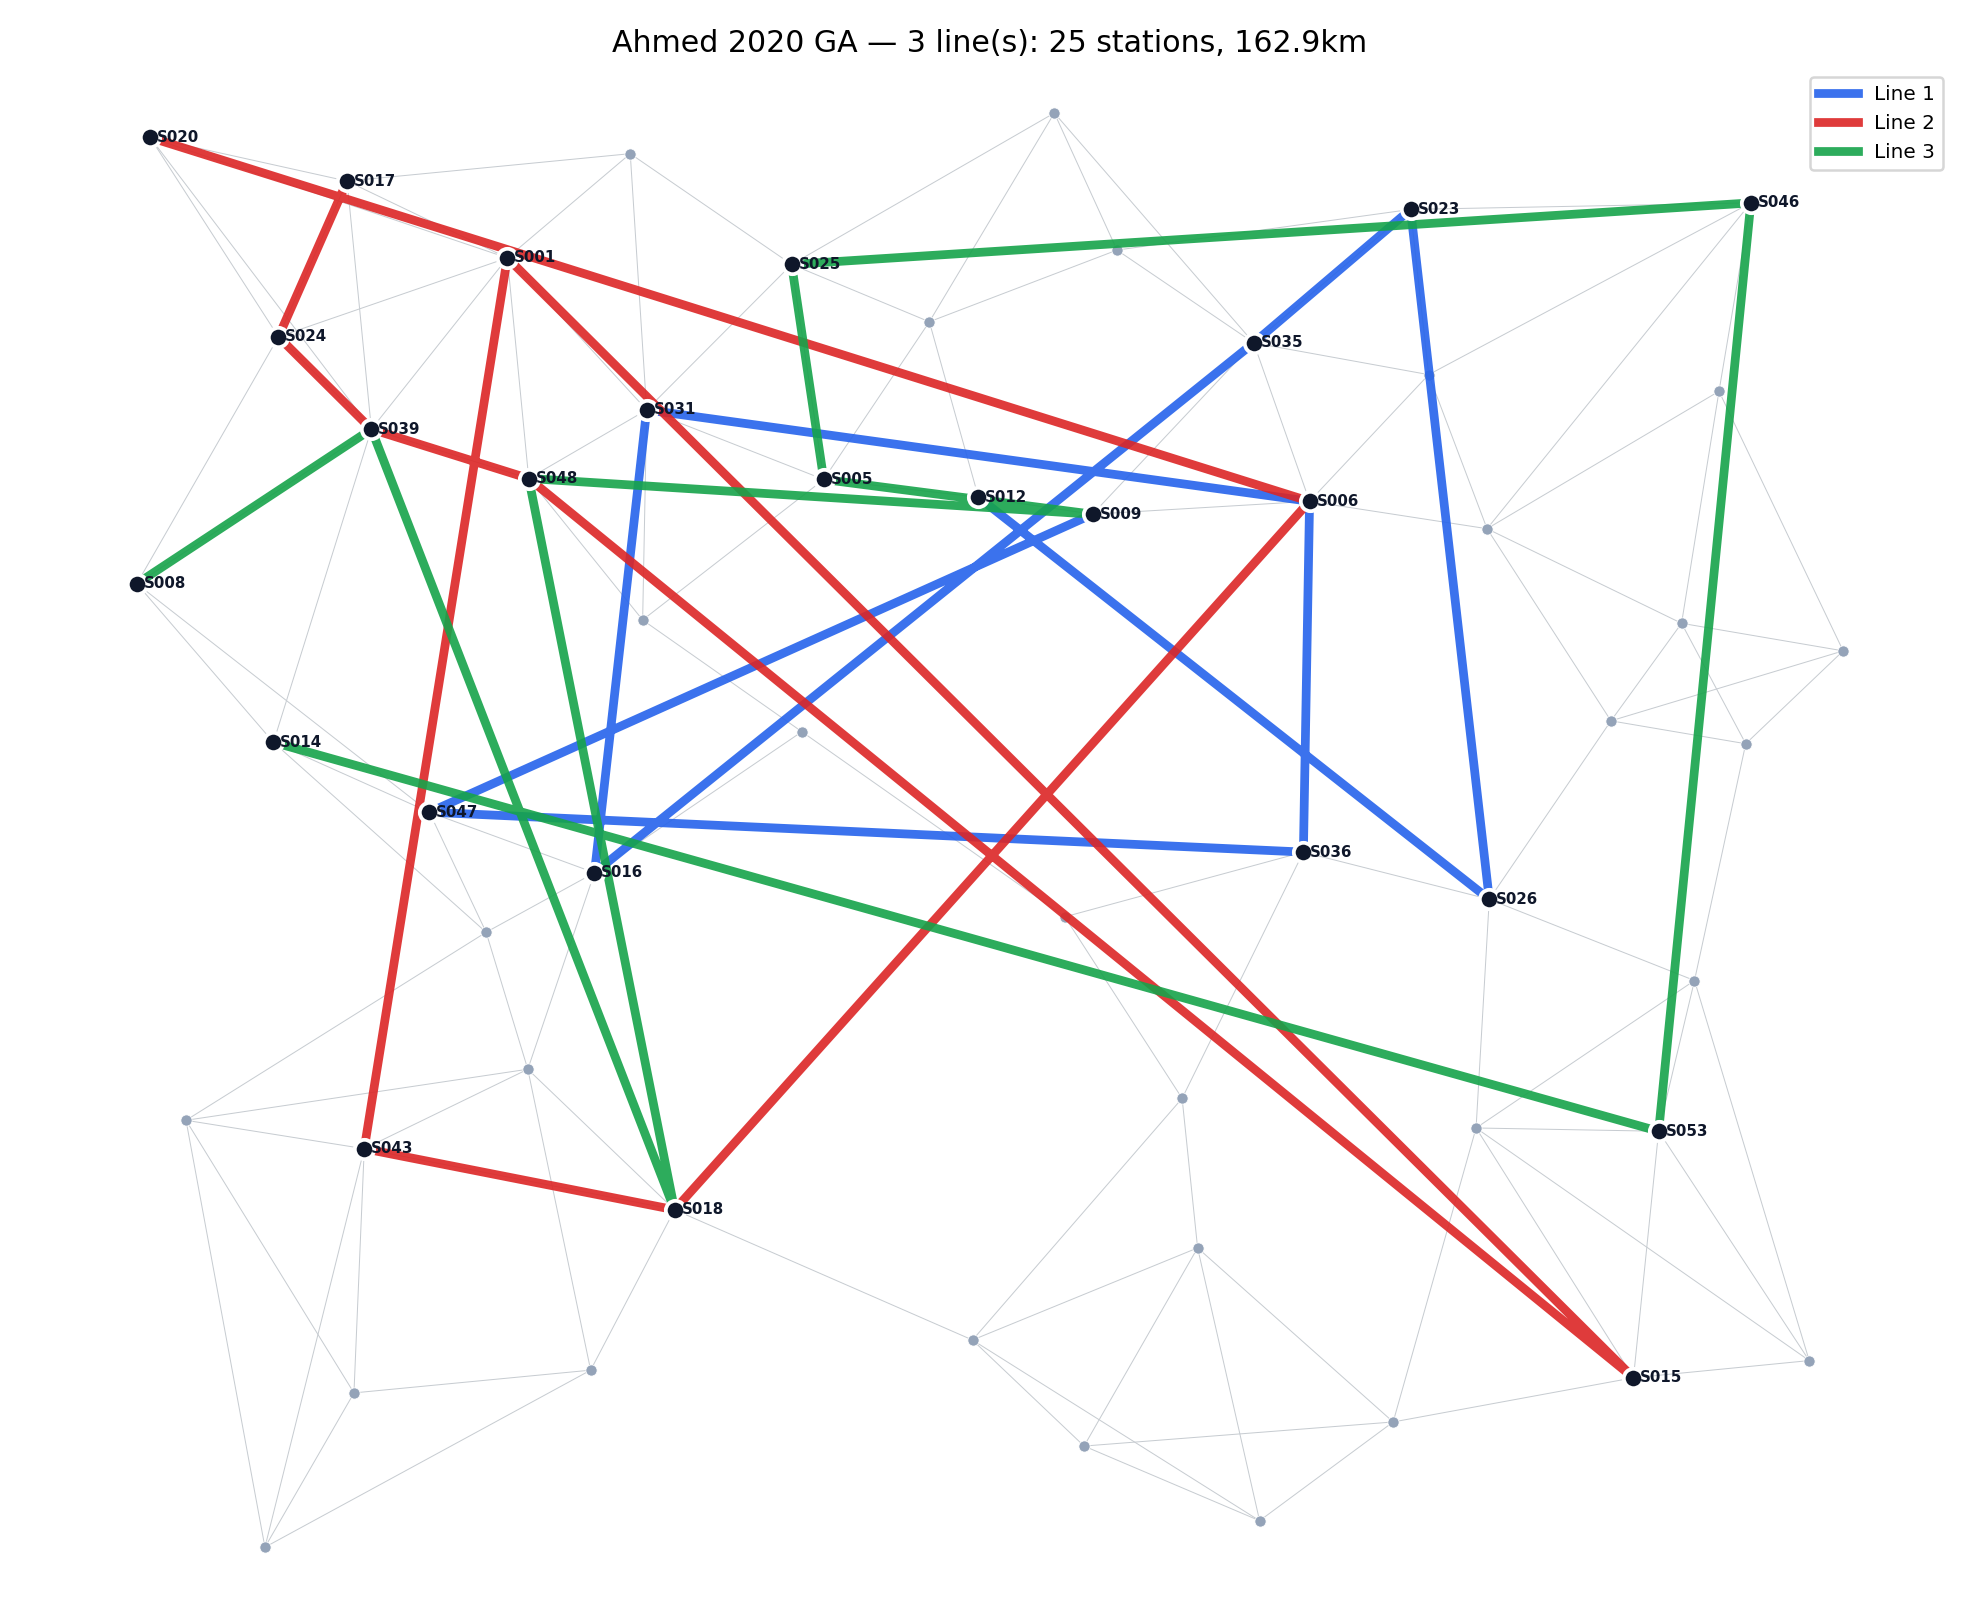
\includegraphics[width=\textwidth]{ahmed2020_reproduction/network_3line}
\end{column}
\end{columns}
\end{frame}

%=======================================================================
\section{Cross-Paper Comparison}
%=======================================================================

%-----------------------------------------------------------------------
\begin{frame}{All Methods Comparison}

\centering
\small
\begin{tabular}{lccccc}
\toprule
\textbf{Method} & \textbf{Stations} & \textbf{Length} & \textbf{OD Coverage} & \textbf{Lines} & \textbf{Runtime} \\
\midrule
Laporte H1    & 18 & 59.8 km & 27.9\% & 1 & 0.05s \\
Laporte H2-A  & 31 & 59.9 km & 54.0\% & 1 & 0.77s \\
Laporte H2-C  & 33 & 59.6 km & 56.8\% & 1 & 0.88s \\
\midrule
Ahmed 1-line  & 14 & 37.0 km & 29.8\% & 1 & 33.5s \\
Ahmed 2-line  & 23 & 85.7 km & 48.9\% & 2 & 56.3s \\
Ahmed 3-line  & 20 & 130.8 km & 31.8\% & 3 & 58.1s \\
\midrule
Greedy-OD     & 23 & 57.1 km & 56.5\% & 3 & 0.01s \\
Greedy-BCR    & 10 & 15.7 km & 27.3\% & 3 & 0.01s \\
GA (line-pool) & 32 & 56.0 km & 40.4\% & 3 & 0.90s \\
\bottomrule
\end{tabular}
\end{frame}

%-----------------------------------------------------------------------
\begin{frame}{Key Findings}

\begin{enumerate}
    \item \textbf{Laporte H2-A/H2-C achieve highest OD coverage} (54--57\%) among all single-line methods.
    \item \textbf{H1 is 25\(\times\) faster} than H2 variants at \(n=100\), but selects fewer stations.
    \item \textbf{Ahmed's multi-line GA} naturally handles transfer stations and network topology.
    \item \textbf{Simultaneous optimization} outperforms individual line design by 18\%.
    \item \textbf{Greedy-OD baseline} is competitive with GA methods at negligible runtime.
\end{enumerate}

\vspace{0.3cm}
\begin{block}{Practical Implication}
For rapid feasibility studies, greedy heuristics suffice. For detailed network design with transfers and multi-line coordination, GA-based methods provide meaningful improvements.
\end{block}
\end{frame}

%-----------------------------------------------------------------------
\begin{frame}{Complexity Comparison}

\centering
\small
\begin{tabular}{lcc}
\toprule
\textbf{Algorithm} & \textbf{Per-Iteration} & \textbf{Total Worst-Case} \\
\midrule
H1 (Laporte)     & \(O(n \cdot |E|^2)\) & \(O(n^2 \cdot |E|^2)\) \\
H2-A/B/C (Laporte) & \(O(n \cdot |E|^3)\) & \(O(n^2 \cdot |E|^3)\) \\
Post-optimization  & \(O(|E|^2 \cdot n)\) per pass & \(O(|E|^3 \cdot n)\) \\
\midrule
Ahmed GA (per gen) & \(O(L \cdot N_s^2 \log N_s)\) & \(O(G \cdot P \cdot L \cdot N_s^2 \log N_s)\) \\
\bottomrule
\end{tabular}

\vspace{0.3cm}
\begin{itemize}
    \item \(n\): stations, \(|E|\): edges, \(L\): lines, \(N_s\): stations per line
    \item \(P\): population, \(G\): generations
    \item All heuristics are \textbf{polynomial-time} despite NP-hard problem.
\end{itemize}
\end{frame}

%=======================================================================
\section{Conclusion}
%=======================================================================

%-----------------------------------------------------------------------
\begin{frame}{Conclusions}

\begin{itemize}
    \item Both papers' algorithms were \textbf{successfully reproduced} on a Shanghai 54-station dataset.
    \item \textbf{Laporte heuristics}: H2 insertion outperforms H1 extension in coverage; H1 wins on speed.
    \item \textbf{Ahmed GA}: simultaneous multi-line optimization is superior to individual line design.
    \item \textbf{Greedy baselines} remain surprisingly competitive for single-objective scenarios.
    \item Deviations from original papers are well-motivated and do not invalidate core algorithmic contributions.
\end{itemize}
\end{frame}

%-----------------------------------------------------------------------
\begin{frame}{Simplifications and Limitations}

\begin{columns}[T]
\begin{column}{0.48\textwidth}
\begin{block}{Simplifications Made}
\begin{itemize}
    \item Gravity-model OD instead of census-tract OD
    \item Pure coverage (\(g_{ij}=1\)) instead of logit mode choice
    \item Simplified 3-component cost (vs.\ 25-equation model)
    \item 54 stations (vs.\ 4774 grid cells)
\end{itemize}
\end{block}
\end{column}
\begin{column}{0.48\textwidth}
\begin{block}{Limitations}
\begin{itemize}
    \item Shanghai data may not generalize to all cities
    \item Simplified cost model may underestimate community costs
    \item No real-world validation of ridership predictions
    \item GA convergence depends on parameter tuning
\end{itemize}
\end{block}
\end{column}
\end{columns}
\end{frame}

%-----------------------------------------------------------------------
\begin{frame}{Future Work}

\begin{itemize}
    \item \textbf{Sensitivity analysis} on Ahmed GA parameters (\(P_c\), \(P_m\), population size)
    \item \textbf{Multi-objective optimization}: Pareto front of coverage vs.\ cost
    \item \textbf{Integration with real transit data}: validate against Shanghai Metro ridership
    \item \textbf{Scalability testing} on larger networks (200+ stations)
    \item \textbf{Hybrid approaches}: use Laporte heuristics to seed the GA population
\end{itemize}
\end{frame}

%-----------------------------------------------------------------------
\begin{frame}{}
\centering
\vspace{1cm}
{\Large\textbf{Thank you!}}\\[0.5cm]
{\large Questions?}

\vspace{1.5cm}
\normalsize
\textit{Code:} \texttt{Rail-Line-Planning/line\_network\_model/}\\[0.2cm]
\textit{Report:} \texttt{doc/report/CS240\_Report.tex}
\end{frame}

\end{document}
